% ------------------------------------------------------------------------------
% TYPO3 CMS 7.2 - What's New - Chapter "Backend User Interface" (English Version)
%
% @author	Michael Schams <schams.net>
% @license	Creative Commons BY-NC-SA 3.0
% @link		http://typo3.org/download/release-notes/whats-new/
% @language	English
% ------------------------------------------------------------------------------
% LTXE-CHAPTER-UID:		93899f32-8efb477e-ed6973d2-b679bd8e
% LTXE-CHAPTER-NAME:	Backend User Interface
% ------------------------------------------------------------------------------
% LTXE-SLIDE-START
% LTXE-SLIDE-UID:		c151f95c-3fe3eb42-442ce244-5f987f80
% LTXE-SLIDE-TITLE:		Customized BE login form
% LTXE-SLIDE-REFERENCE:	unknown
% ------------------------------------------------------------------------------
\begin{frame}[fragile]
	\frametitle{Backend User Interface}
	\framesubtitle{Customisable Login Form}

	System extension \texttt{backend} allows administrators to configure a custom
	background image, a logo and a colour for the backend login screen:

	\begin{figure}
		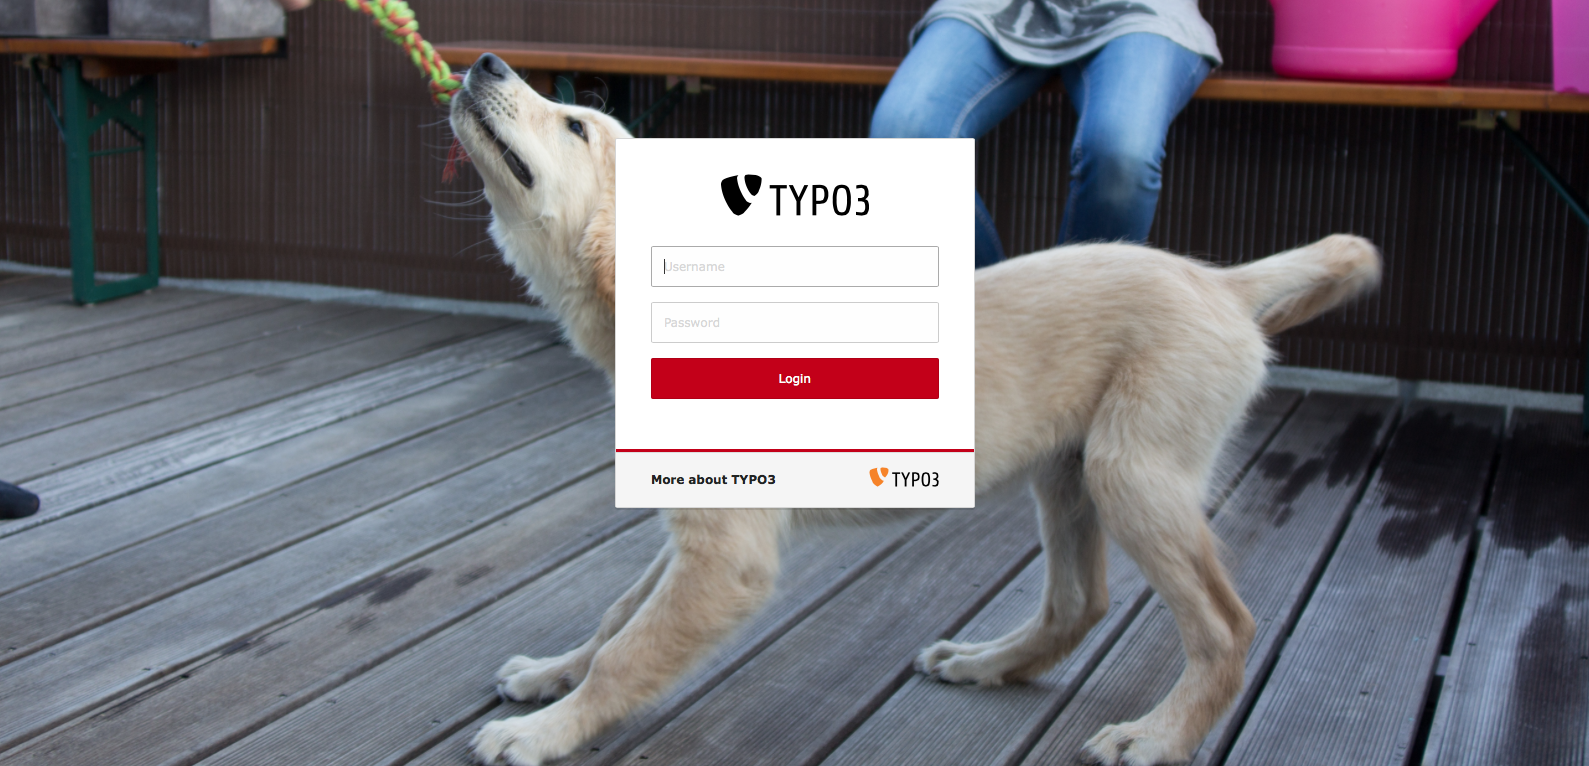
\includegraphics[width=0.75\linewidth]{BackendUserInterface/Login.png}
	\end{figure}

\end{frame}

% ------------------------------------------------------------------------------
% LTXE-SLIDE-START
% LTXE-SLIDE-UID:		e2e353ae-3b2b5c00-0cd7c57d-d97d22c9
% LTXE-SLIDE-TITLE:		Add image cropping
% LTXE-SLIDE-REFERENCE:	Feature-65584-AddImageCropping.rst
% ------------------------------------------------------------------------------
\begin{frame}[fragile]
	\frametitle{Backend User Interface}
	\framesubtitle{Image Manipulation: Cropping}

	An image manipulation functionality allows editors to crop images in the backend.
	This feature must be explicitly activated for BE users ("Exclude Fields"):

	\begin{figure}
		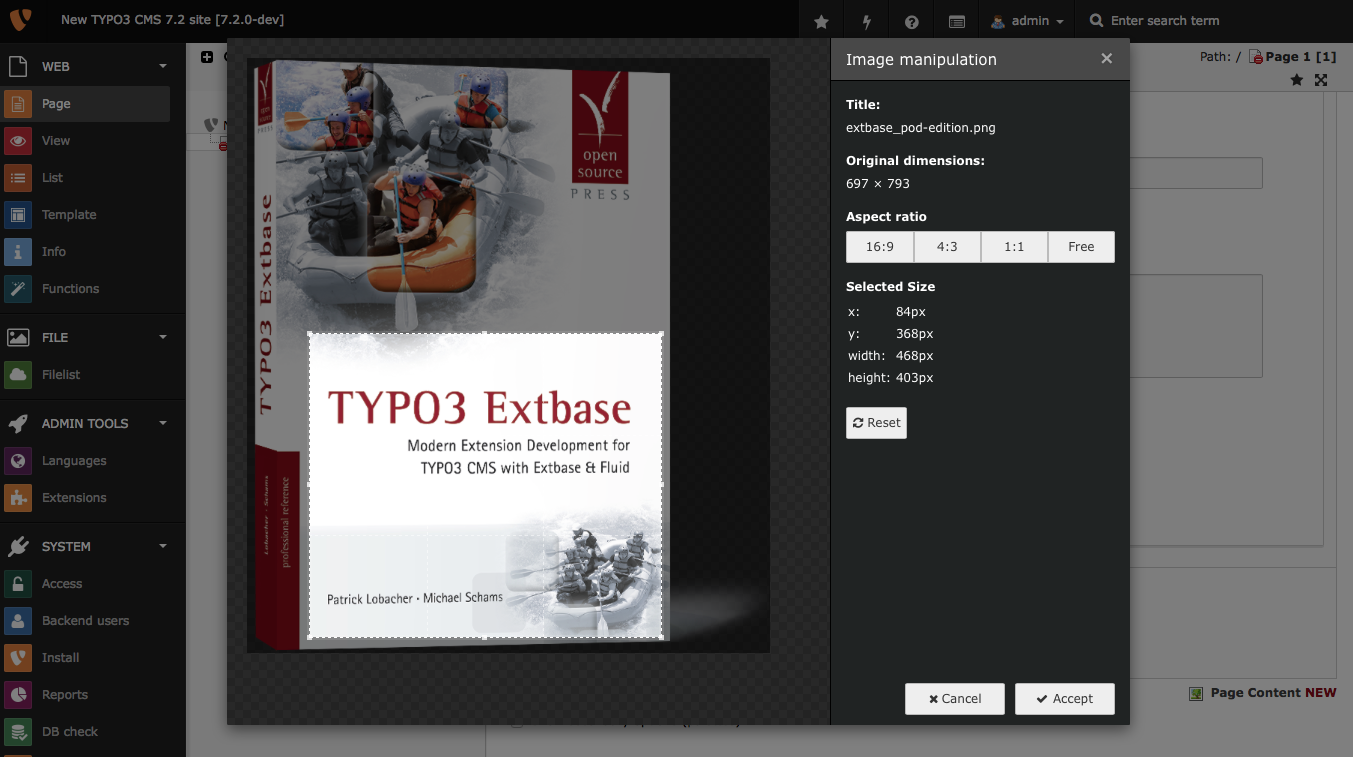
\includegraphics[width=0.7\linewidth]{BackendUserInterface/ImageCropping.png}
	\end{figure}

\end{frame}

% ------------------------------------------------------------------------------
% LTXE-SLIDE-START
% LTXE-SLIDE-UID:		301dfea9-d2debf3e-dcaa7bcd-205e5990
% LTXE-SLIDE-TITLE:		Add backend user groups to backend user module
% LTXE-SLIDE-REFERENCE:	Feature-64686-AddBackendUserGroupsToBackendUserModule.rst
% ------------------------------------------------------------------------------
\begin{frame}[fragile]
	\frametitle{Backend User Interface}
	\framesubtitle{Backend User Groups}

	Backend user groups can be maintained in a submodule of the "Backend Users" module now:

	\begin{figure}
		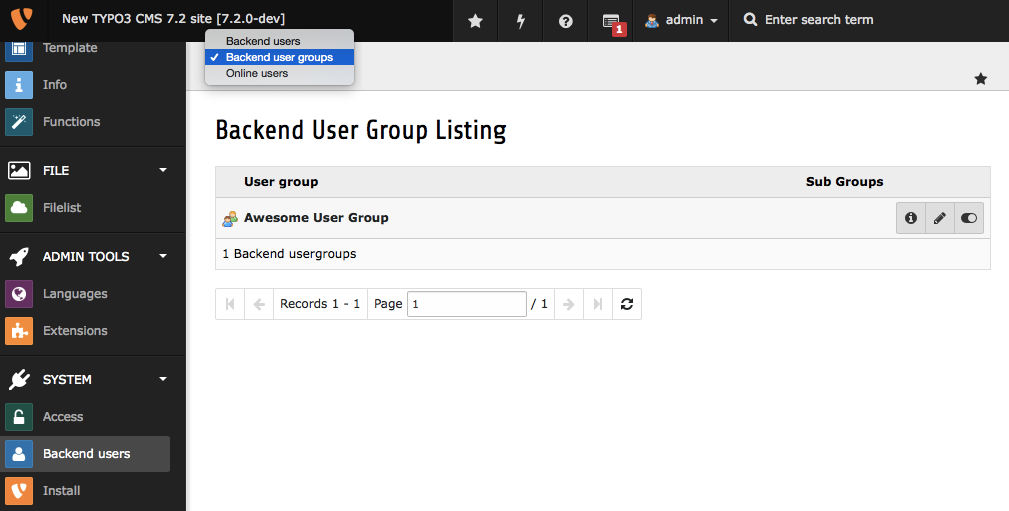
\includegraphics[width=0.70\linewidth]{BackendUserInterface/UserGroups.png}
	\end{figure}

\end{frame}

% ------------------------------------------------------------------------------
% LTXE-SLIDE-START
% LTXE-SLIDE-UID:		daa83c1e-08d2716b-de74cbda-42361551
% LTXE-SLIDE-TITLE:		Extension Manager: Disable automatic installation
% LTXE-SLIDE-REFERENCE:	Feature-50501-DisableAutomaticExtInstallation.rst
% ------------------------------------------------------------------------------
\begin{frame}[fragile]
	\frametitle{Backend User Interface}
	\framesubtitle{Disable Automatic Extension Installation}

	Administrators can configure the Extension Manager not to install downloaded
	extensions straight away:

	\begin{figure}
		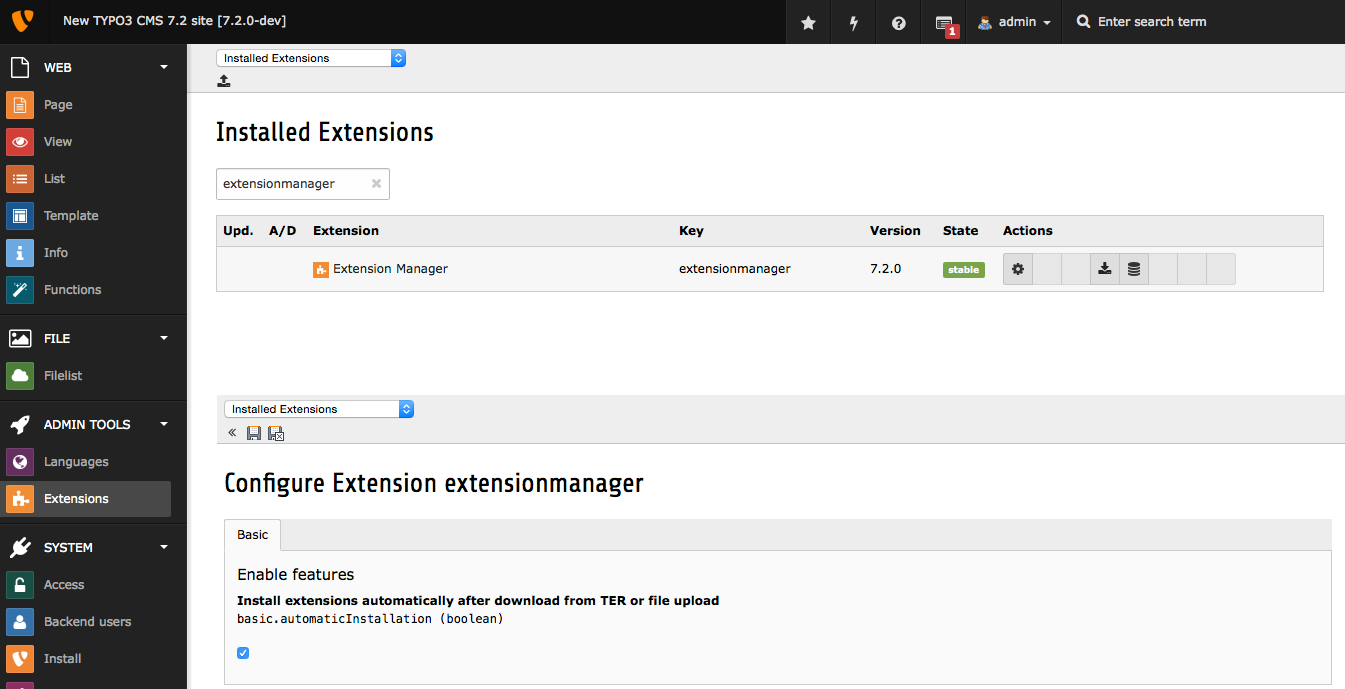
\includegraphics[width=0.70\linewidth]{BackendUserInterface/ExtManager.png}
	\end{figure}

\end{frame}

% ------------------------------------------------------------------------------
% LTXE-SLIDE-START
% LTXE-SLIDE-UID:		20769920-da9df227-c3b527b9-9a23bac1
% LTXE-SLIDE-TITLE:		Show remaining characters below text fields
% LTXE-SLIDE-REFERENCE:	Feature-66029-ShowRemainingCharactersBelowTextFields.rst
% ------------------------------------------------------------------------------
\begin{frame}[fragile]
	\frametitle{Backend User Interface}
	\framesubtitle{Remaining Characters on Text Fields}

	The number of remaining characters is displayed below text input fields:

	\begin{figure}
		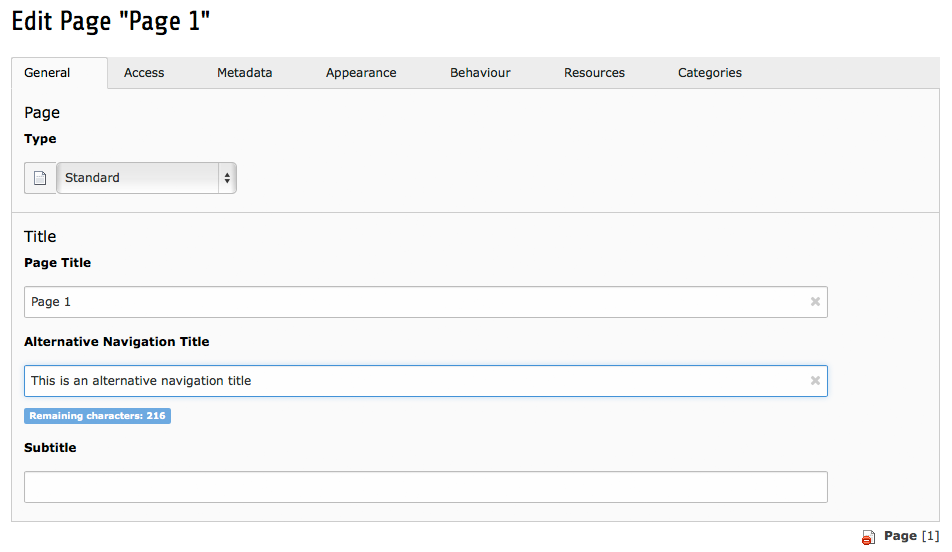
\includegraphics[width=0.70\linewidth]{BackendUserInterface/RemainingCharacters.png}
	\end{figure}

\end{frame}

% ------------------------------------------------------------------------------
% LTXE-SLIDE-START
% LTXE-SLIDE-UID:		ff760b86-9d6b1ecd-d0e98565-f23c51f0
% LTXE-SLIDE-TITLE:		Show confirm message on closing an editform with unsaved changes
% LTXE-SLIDE-REFERENCE:	Feature-65996-AddConfirmationOnCloseEditformWithUnsavedChanges.rst
% ------------------------------------------------------------------------------
\begin{frame}[fragile]
	\frametitle{Backend User Interface}
	\framesubtitle{Confirm Unsaved Changes}

	A new confirmation dialog warns editors about loosing unsaved changes:

	\begin{figure}
		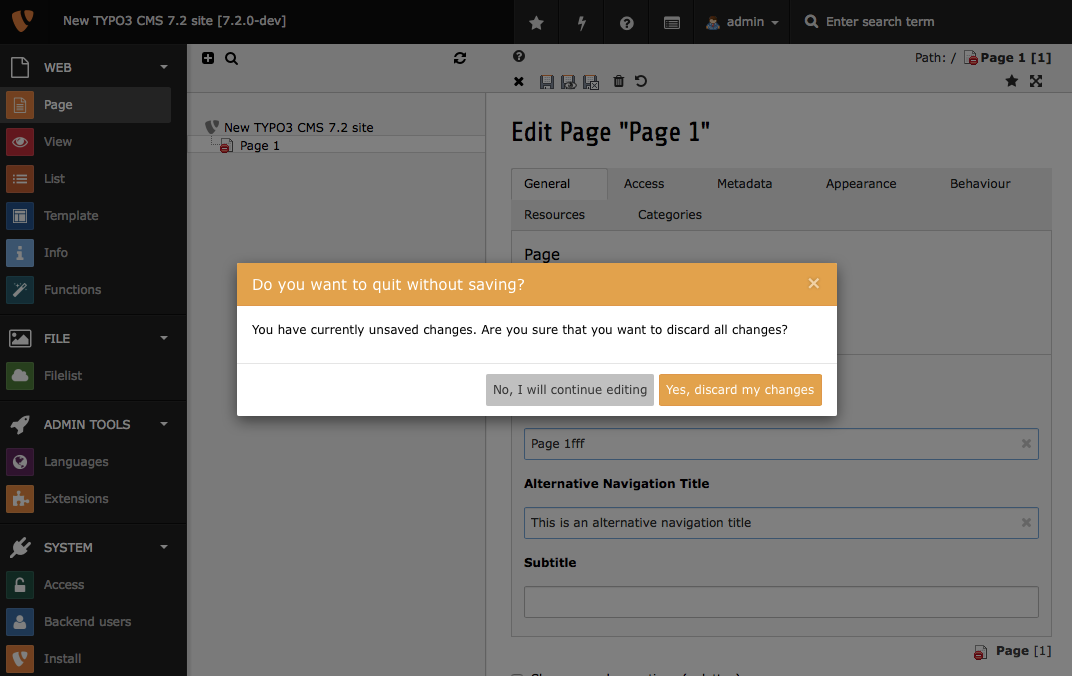
\includegraphics[width=0.65\linewidth]{BackendUserInterface/ClosingDialog.png}
	\end{figure}

\end{frame}

% ------------------------------------------------------------------------------
% LTXE-SLIDE-START
% LTXE-SLIDE-UID:		6ac9a35e-46541895-7509263e-28fb799f
% LTXE-SLIDE-TITLE:		System Information Dropdown
% LTXE-SLIDE-REFERENCE:	Feature-65767-SystemInformationDropdown.rst
% ------------------------------------------------------------------------------
\begin{frame}[fragile]
	\frametitle{Backend User Interface}
	\framesubtitle{System Information Dropdown}

	A dropdown menu shows several information about the system TYPO3 is installed on.
	The data of this dialog can be extended:\newline
	\small(see chapter "In-Depth Changes" for further details)\normalsize

	\begin{figure}
		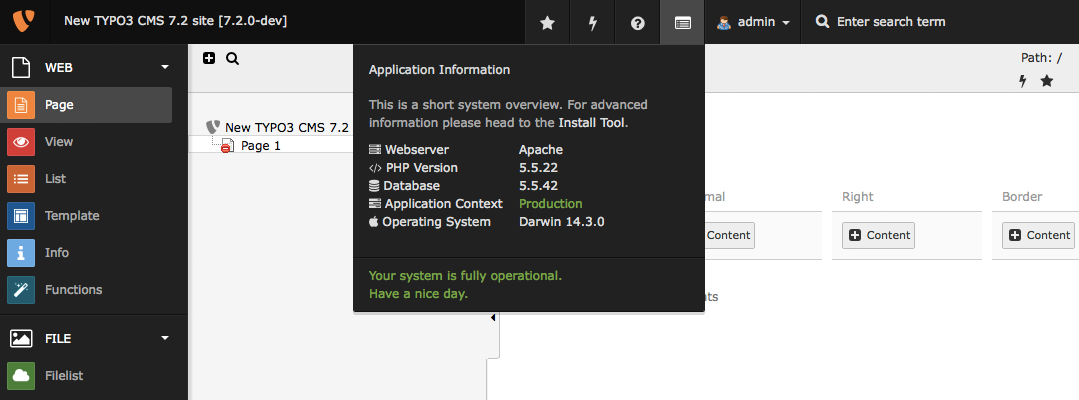
\includegraphics[width=0.85\linewidth]{BackendUserInterface/SystemInformation.png}
	\end{figure}

\end{frame}

% ------------------------------------------------------------------------------
% LTXE-SLIDE-START
% LTXE-SLIDE-UID:		79a2ee0c-3439d600-08990adb-6bed8c19
% LTXE-SLIDE-TITLE:		Ask for old password when changing
% LTXE-SLIDE-REFERENCE:	commit bf6f5226eb6cb441bb53657a88ef42f1cdb5155f
% ------------------------------------------------------------------------------
\begin{frame}[fragile]
	\frametitle{Backend User Interface}
	\framesubtitle{Changing Password}

	Backend users are forced to provide the current (old) password in order to change
	it to a new password:

	\begin{figure}
		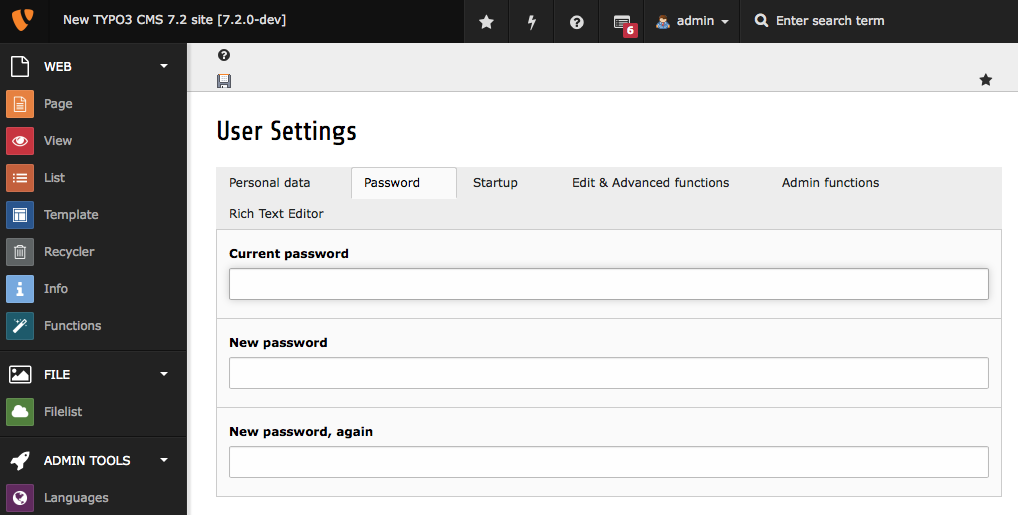
\includegraphics[width=0.7\linewidth]{BackendUserInterface/Password.png}
	\end{figure}

\end{frame}

% ------------------------------------------------------------------------------
% LTXE-SLIDE-START
% LTXE-SLIDE-UID:		7725bce9-e606f055-bf2e7b4a-e870fe2a
% LTXE-SLIDE-TITLE:		Add icon for "Show Content From Page"
% LTXE-SLIDE-REFERENCE:	commit f8aa3eea9aed97a901ef0c3e7c650e1218839596
% ------------------------------------------------------------------------------
\begin{frame}[fragile]
	\frametitle{Backend User Interface}
	\framesubtitle{Page Icon for "Show Content from Page"}

	A new page icon in the page tree indicates that a page shows content from another page:

	\begin{figure}
		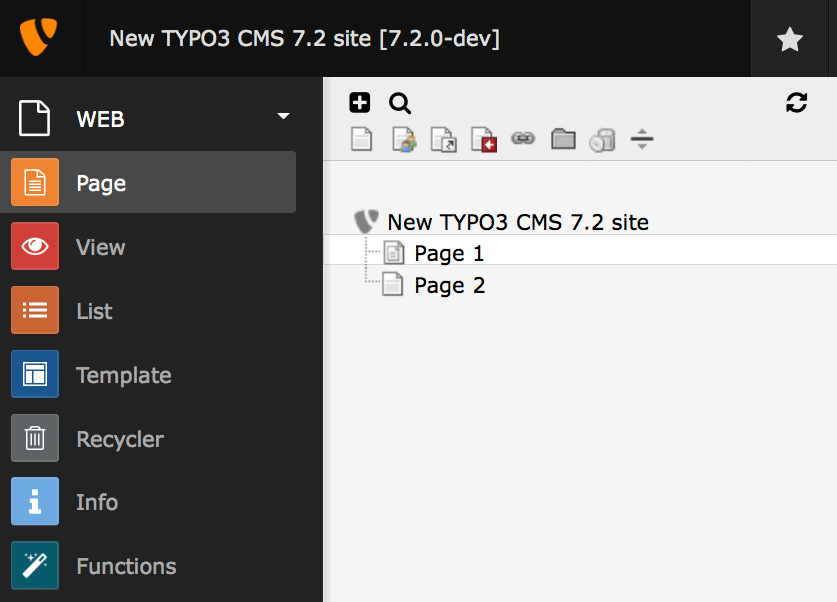
\includegraphics[width=0.45\linewidth]{BackendUserInterface/ShowContent.png}
	\end{figure}

\end{frame}

% ------------------------------------------------------------------------------
% LTXE-SLIDE-START
% LTXE-SLIDE-UID:		5ac2de45-9be12bf9-1c326192-602839fb
% LTXE-SLIDE-TITLE:		Extension Manager: Choose version for update
% LTXE-SLIDE-REFERENCE:	commit a26396a4530b530744ec8b36c5fb5606789a6739
% ------------------------------------------------------------------------------
\begin{frame}[fragile]
	\frametitle{Backend User Interface}
	\framesubtitle{Extension Updates}

	When updating an extension, it is now possible to choose the target version:

	\begin{figure}
		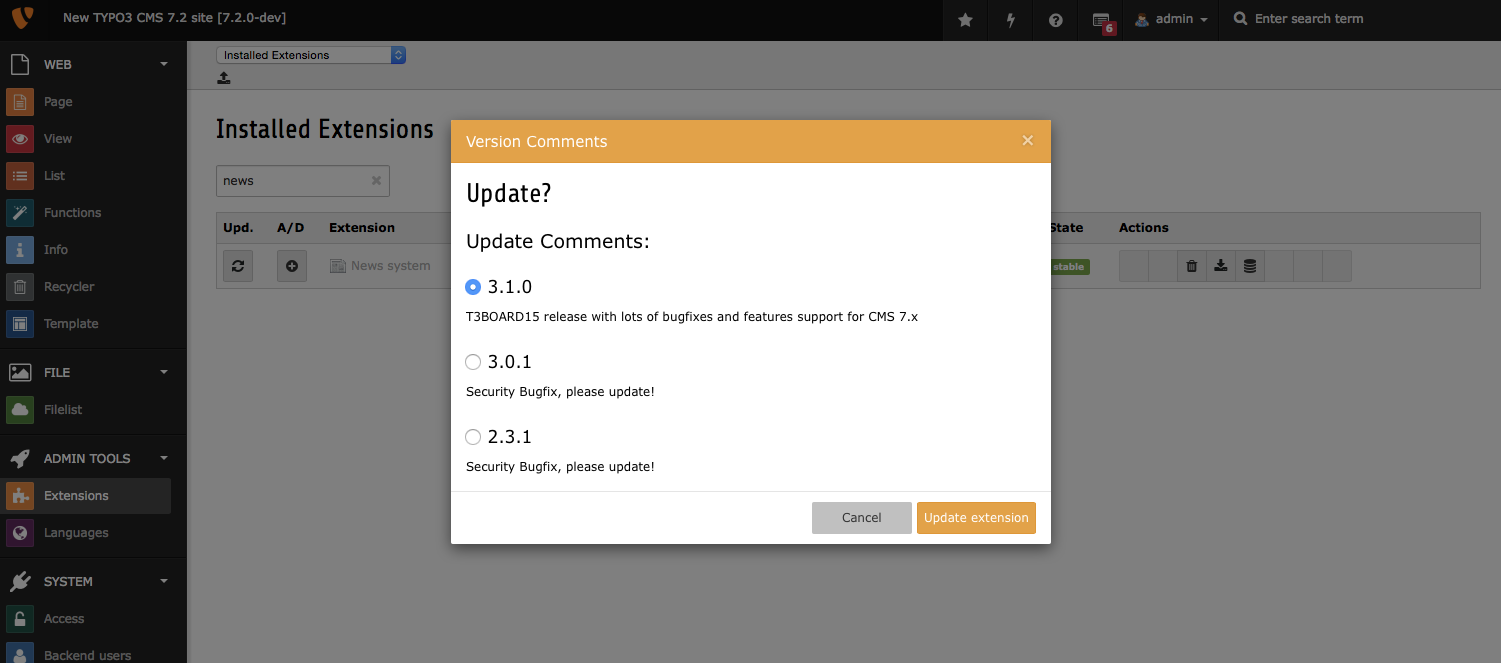
\includegraphics[width=0.75\linewidth]{BackendUserInterface/Update.png}
	\end{figure}

\end{frame}

% ------------------------------------------------------------------------------
% LTXE-SLIDE-START
% LTXE-SLIDE-UID:		f6be31f7-155d676c-0e551545-3fc89e89
% LTXE-SLIDE-TITLE:		Add scheduler task to remove deleted records
% LTXE-SLIDE-REFERENCE:	Feature-32651-AddSchedulerTaskToRemoveDeletedRecords.rst
% ------------------------------------------------------------------------------
\begin{frame}[fragile]
	\frametitle{Backend User Interface}
	\framesubtitle{Recycler Task}

	A new scheduler task for system extension \texttt{recycler} removes deleted
	records from content tables in the database. The maximum age and the affected
	tables are configurable in the task's settings.
	\newline
	This may also apply to files, if they are referenced in the content element.

	\begin{figure}
		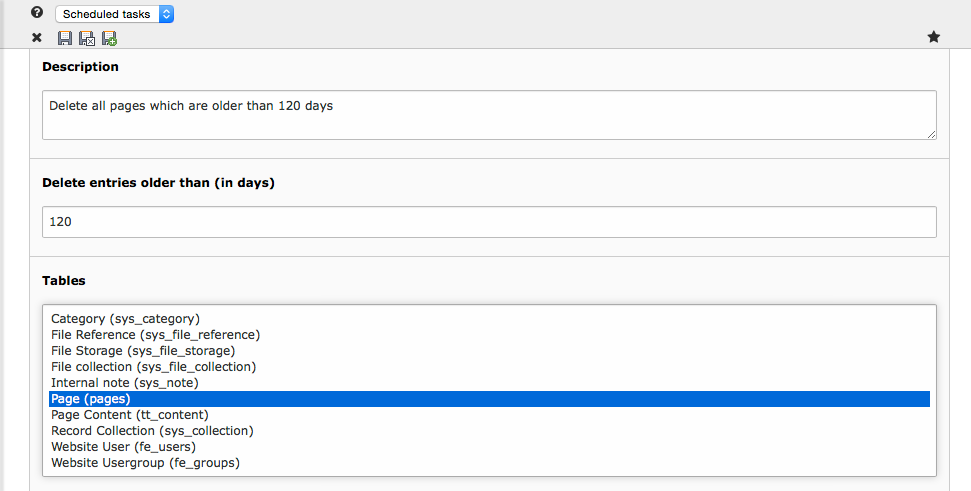
\includegraphics[width=0.68\linewidth]{BackendUserInterface/RecyclerTask.png}
	\end{figure}

\end{frame}

% ------------------------------------------------------------------------------
